%%%%%%%%%%%%%%%%%%%%%%%%%%%%%%%%%%%%%%%%%
% Beamer Presentation
% LaTeX Template
% Version 1.0 (10/11/12)
%
% This template has been downloaded from:
% http://www.LaTeXTemplates.com
%
% License:
% CC BY-NC-SA 3.0 (http://creativecommons.org/licenses/by-nc-sa/3.0/)
%
%%%%%%%%%%%%%%%%%%%%%%%%%%%%%%%%%%%%%%%%%

%----------------------------------------------------------------------------------------
%	PACKAGES AND THEMES
%----------------------------------------------------------------------------------------

\documentclass{beamer}

\mode<presentation> {

% The Beamer class comes with a number of default slide themes
% which change the colors and layouts of slides. Below this is a list
% of all the themes, uncomment each in turn to see what they look like.
%\usetheme{Berkeley}4
\usetheme{CambridgeUS}
%\usetheme{PaloAlto}4

% As well as themes, the Beamer class has a number of color themes
% for any slide theme. Uncomment each of these in turn to see how it
% changes the colors of your current slide theme.

%\usecolortheme{beaver}4
\usecolortheme{lily}
%\usecolortheme{orchid}4
%\usecolortheme{wolverine}4

%\setbeamertemplate{footline} % To remove the footer line in all slides uncomment this line
%\setbeamertemplate{footline}[page number] % To replace the footer line in all slides with a simple slide count uncomment this line

%\setbeamertemplate{navigation symbols}{} % To remove the navigation symbols from the bottom of all slides uncomment this line
}

\usepackage{amsmath,amssymb,amsfonts,amsthm}
\usepackage{etex} % Needed in the newest version in order to compile properly
\usepackage{lmodern} % Needed in the newest version in order to compile properly
\usepackage{graphicx} % Allows including images
\usepackage{booktabs} % Allows the use of \toprule, \midrule and \bottomrule in tables
\usepackage{tikz}
\usepackage{tikz-qtree}
\usetikzlibrary{trees} % This is to allow the fork right path
\theoremstyle{definition}
%\newtheorem{theorem}[theorem]{Theorem}

%----------------------------------------------------------------------------------------
%	TITLE PAGE
%----------------------------------------------------------------------------------------

\title[Data Compression]{Huffman Algorithm for Data Compression} % The short title appears at the bottom of every slide, the full title is only on the title page

\author{N. Cortez, A. Martinez, J. Mota, J. Westcott} % Your name
\date{\today} % Date, can be changed to a custom date

\begin{document}

%frame 1
\begin{frame}
\titlepage % Print the title page as the first slide
\end{frame}

%frame 2
\begin{frame}

\frametitle{Overview} % Table of contents slide, comment this block out to remove it
\tableofcontents % Throughout your presentation, if you choose to use \section{} and \subsection{} commands, these will automatically be printed on this slide as an overview of your presentation
\section{History}
\section{Data Compression}
\section {Probability Theory}
\section {Entropy}
\section{Huffman Algorithm}
\section{Analysis of Results}

\end{frame}

%frame 3
\begin{frame}

\frametitle{History}

\begin{figure}

\centering
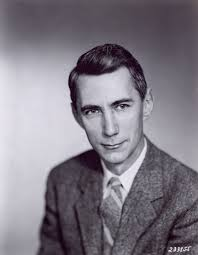
\includegraphics[scale=0.4]{Claude_Shannon}

\end{figure}

In 1938, Claude Shannon solidified the branch of information theory through his groundbreaking master's thesis, \textit{A Symbolic Analysis of Relay and Switching Circuits}.  In his thesis, Shannon demonstrated how to measure information by instituting a relationship between symbolic logic and relay circuits. Moreover, his thesis established the concept of information entropy, measuring the information gained from observing a random variable. 

\end{frame}

%frame 4
\begin{frame}

\frametitle{History}

One application of information theory is data compression. David Huffman, an MIT graduate, was given the option of taking a final exam or writing a research paper on an efficient binary compression code as a final project in one of his graduate courses. Huffman chose the latter and created what was to be known as the Huffman Algorithm. His algorithm addressed the issue of how to reduce redundancy in an input message by encoding it in as few bits, or pieces of information, as possible. 

\end{frame}

%frame 5
\begin{frame}

\frametitle{What is Data Compression?}

\begin{definition}[Data Compression]
The technique in information theory by which the same amount of data is transmitted via a smaller number of bits. This is useful for truncating information and transporting it near real time.
\end{definition}

\pause

\begin{center}
\begin{tabular}{ | l | l|  }
\hline
Lossless & Lossy \\ \hline
PNG & JPEG \\
FLAC & MP3 \\
QuickTime Animation & MPEG \\
\hline
\end{tabular}
\end{center}

\end{frame}

% frame 6
\begin{frame}

\frametitle{Probability Theory: The Basics}
In order to understand data compression one must have a foundation in elementary probability theory.
Note that the probability of the values of a random variable will satisfy a probability distribution.

\pause

\begin{definition}[Random Variable]
A variable whose value is subject to variations due to chance.
\end{definition}

\pause

\begin{definition}[Expected Value]
The weighted sum of the possible values of a random variable with their respective probabilities so that: \\\center$E[x]=\sum\limits_{i=1}^{n}{x_{i}P(x_{i})}$.
\end{definition}

\end{frame}

% frame 7
\begin{frame}

\frametitle{Entropy}
\begin{definition}[Entropy]
The expected value of the information content, $-log(P(X))$, of a random variable found by: \[E\left[-log(P(X))\right]=\sum_{i=1}^{n}{{p_{i}}(-log(p_{i}))},\] where the random variable $X$ takes values $x_{1},x_{2},\ldots,x_{n}$ with associated probabilities $p_{1},p_{2},\ldots,p_{n}.$
\end{definition}

\pause

Example:
\begin{table}
\parbox{.4\linewidth}{
\hspace{1.5cm}{Fair Coin} \\E=1
\centering
\begin{tabular}{|c|c|c|}
\hline
x & p(x) \\ \hline
Heads & 1/2 \\
\hline
Tails & 1/2 \\
\hline
\end{tabular}
}
\parbox{.49\linewidth}{
\hspace{1.7cm}{Biased Coin} \\E=0
\centering
\begin{tabular}{|c|c|c|}
\hline
x & p(x) \\ \hline
Heads & 1 \\
\hline
Tails & 0 \\
\hline
\end{tabular}
}
\end{table}

\end{frame}

% frame 8
\begin{frame}

\frametitle{Entropy: Relevancy}
\begin{theorem}[Shannon's Coding Theorem]
Let $X$ be a random variable with $n$ possible letters and entropy: \\ $H(X)=\sum_{i=1}^{n}{{p_{i}}(-log(p_{i}))}$. Let $L$ be the average number of bits to encode $N$ symbols selected randomly with X. Then for the optimal coding:
\begin{displaymath}
H(X) \leq L < H(X) + \frac{1}{N}
\end{displaymath}

\end{theorem}

This theorem establishes the relationship between the entropy and the average length of code. Shannon proved that the entropy is the best average length of code that could possibly be reached. He also demonstrated that one may get arbitrarily close to the entropy and so this establishes a lower bound on how efficient lossless codes may be.

\end{frame}

% frame 9
\begin{frame}

\frametitle{Huffman Algorithm}
\begin{definition}[The Huffman Algorithm]
A compression algorithm that allows us to give letters with lower probability longer code words and letters with higher probability shorter code words.
\end{definition}

David Huffman showed that you can find a code for a given text whose average length can get close to the entropy without losing information.

\end{frame}

% frame 10

\begin{frame}

\frametitle{Huffman Algorithm: Example}

\center
Text: ACCDEEEFAFECEEEB

\pause

\begin{center}
\begin{tabular}{ | l | l | }
\hline
x & p(x) \\ \hline
A & 2/16 \\ \hline
B & 1/16 \\ \hline
C & 3/16 \\ \hline
D & 1/16 \\ \hline
E & 7/16 \\ \hline
F & 2/16 \\
\hline
\end{tabular}
\end{center}

\end{frame}

% frame 11
\begin{frame}

\frametitle{Huffman Algorithm: Example}

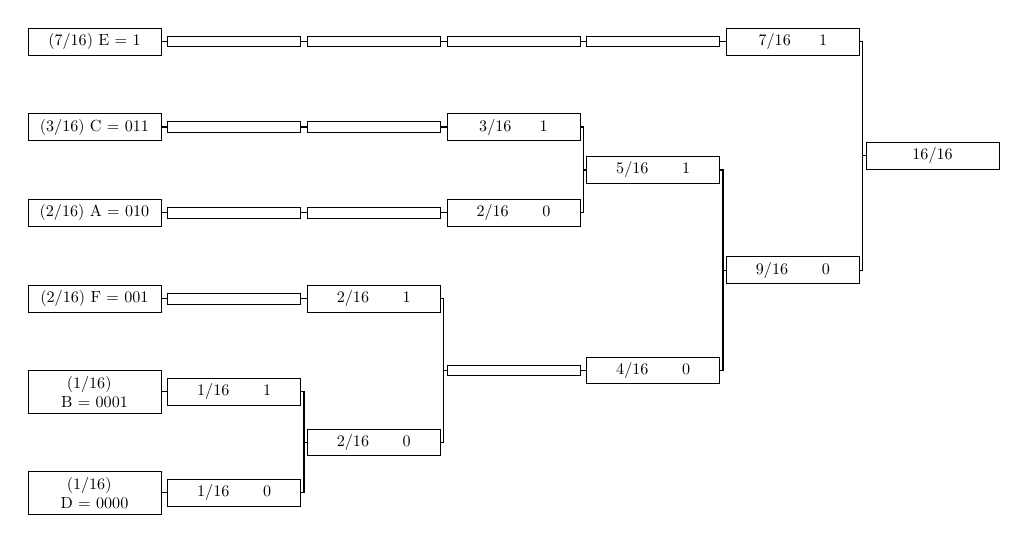
\begin{tikzpicture}[level distance=1.2in,sibling distance=.5in,scale=.582]
\tikzset{edge from parent/.style= 
            {thick, draw,
                edge from parent fork right},every tree node/.style={draw,minimum width=.75in,text width=1in, align=center},grow'=right}

\begin{scope}
\tikzset{edge from parent/.style= 
            {thick, draw,
                edge from parent fork left},every tree node/.style={draw,minimum width=1.05in,text width=1.05in, align=center},grow'=left}

\Tree 
    [. 16/16
        [. {9/16 \hspace{.5 cm} 0}
       		[.{4/16 \hspace{.5 cm} 0 }
			[. {}	
				[.{2/16 \hspace{.5 cm} 0 } 
				[.{ 1/16 \hspace{.5 cm} 0 }
					[. {\hspace{.73cm}(1/16) \newline D = 0000} ]
				 ]
				[.{ 1/16 \hspace{.5 cm} 1 }
					[. {\hspace{.73cm}(1/16) \newline B = 0001} ]
				 ]
				]
				[.{ 2/16 \hspace{.5 cm} 1 }
					[. {}
						[. {$(2/16)$  F = 001} ]
			           	 ]
				 ]
			]
		 ]
		[.{5/16 \hspace{.5 cm} 1 } 
			[.{ 2/16 \hspace{.5 cm} 0 } 	
				[. {}
					[. {}
						[. {(2/16) A = 010} ]
					 ]
				]
			]
			[.{ 3/16 \hspace{.5 cm}1}
				[. {}
					[. {}
						[. {(3/16) C = 011} ]
					]
				 ]
			]
		]
	]
	[. {7/16 \hspace{.5 cm}1}
		[. {}
	 		[. {}
				 [. {}
					[. {}
						[. {(7/16)  E = 1} ]
					]
			 	]
	 		]
	 	]
	]
    ]

\end{scope}

\end{tikzpicture}

\end{frame}

% frame 12
\begin{frame}

\frametitle{What We Did}

\center
\Large
We made our own implementation of Huffman's Algorithm in a C++ program. We then tested this on different types of files composed of a variety of sizes.

\end{frame}

% frame 13
\begin{frame}

\frametitle{Analysis of Results}

\begin{center}
\begin{tabular}{ | l | l | l | l | }
\hline
 & Makefile & Small Text & Circle Image \\ \hline
Original Size (Bytes) & 343 & 20 & 52958 \\ \hline
Compressed Size (Bytes) & 291 & 41 & 46059 \\ \hline
Average Word Size & 4.5889 & 3.85 & 6.8748 \\ \hline
Entropy & 4.5666 & 3.7842 & 6.8468 \\ \hline
Min. Possible Size (Bytes) & 195.79 & 9.4605 & 45323 \\ \hline
\end{tabular}
\end{center}

\begin{center}
\begin{tabular}{ | l | l | l | l | }
\hline
 & Source Code & Scream Audio & Large Text \\ \hline
Original Size (Bytes) & 15249 & 1004656 & 316794 \\ \hline
Compressed Size (Bytes) & 8586 & 851056 & 182234 \\ \hline
Average Word Size & 4.3965 & 6.7725 & 4.5966 \\ \hline
Entropy & 4.3375 & 6.7304 & 4.5653 \\ \hline
Min. Possible Size (Bytes) & 8267.9 & 845216 & 180782 \\ \hline
\end{tabular}
\end{center}

\end{frame}

% frame 14
\begin{frame}

\frametitle{References}

D. Salomon, \textit{Data Compression: The Complete Reference}, Springer, New York, NY, USA, 4th edition, 2007.
\vspace{.5 cm}

D. A. Huffman, "A Method for the Construction of Minimum Redundancy Codes," \textit{Proceedings of the Institute of Radio Engineers}, vol. 40, no. 9, pp. 1098-1101, 1952.
\vspace{.5 cm}

Lee, Joseph, "Huffman Data Compression," \textit{MIT Undergraduate Journal of Mathematics}, May 23, 2007.
\vspace{.5 cm}

Shannon, C. E. \& Weaver, W., \textit{The Mathematical Theory of Communication}. Urbana, IL: University of Illinois Press, 1949.

\end{frame}

% frame 15
\begin{frame}

\center
\Huge
Thank you!

\end{frame}

\end{document} 